\documentclass[nocopyrightspace]{sigplanconf}
\usepackage{url}
\usepackage{stmaryrd}
\usepackage{epsfig}
\usepackage{alltt}
\usepackage{times}
\usepackage{code}
\usepackage{xspace}

\renewcommand{\floatpagefraction}{0.9}

\newcommand{\cut}[1]{}

\newcommand{\appref}[1]{Appendix~\ref{#1}}
\newcommand{\secref}[1]{Section~\ref{#1}}
\newcommand{\tblref}[1]{Table~\ref{#1}}
\newcommand{\figref}[1]{Figure~\ref{#1}}
\newcommand{\listingref}[1]{Listing~\ref{#1}}
%\newcommand{\pref}[1]{{page~\pageref{#1}}}

\newcommand{\eg}{{\em e.g.}}
\newcommand{\cf}{{\em cf.}}
\newcommand{\ie}{{\em i.e.}}
\newcommand{\etc}{{\em etc.\/}}
\newcommand{\naive}{na\"{\i}ve}
\newcommand{\role}{r\^{o}le}
\newcommand{\forte}{{fort\'{e}\/}}
\newcommand{\appr}{\~{}}

\newcommand{\bftt}[1]{{\ttfamily\bfseries{}#1}}
\newcommand{\kw}[1]{\bftt {#1}}
\newcommand{\Pthen}{\kw{Pthen}}
\newcommand{\pads}{\textsc{pads}}
\newcommand{\padsl}{\textsc{padsl}}
\newcommand{\padst}{\textsc{pads/t}}
\newcommand{\datatype}{\textsc{PADS/T}}
%\newcommand{\datatype}{\textsc{DataType}}
\newcommand{\C}{\textsc{C}}
\newcommand{\perl}{\textsc{Perl}}
\newcommand{\ml}{\textsc{ml}}
\newcommand{\sml}{\textsc{sml}}
\newcommand{\smlnj}{\textsc{sml/nj}}
\newcommand{\java}{\textsc{java}}
\newcommand{\ddl}{\textsc{ddl}}
\newcommand{\xml}{\textsc{xml}}
\newcommand{\datascript}{\textsc{DataScript}}
\newcommand{\packettypes}{\textsc{PacketTypes}}
\newcommand{\erlang}{\textsc{Erlang}}

\newcommand{\Core}{Ad hoc}
\newcommand{\core}{ad hoc}
\newcommand{\pvalue}{\core{} value}
\newcommand{\ppat}{\core{} pattern}
\newcommand{\ptype}{\core{} type}

\newcommand{\padsc}{\textsc{pads}/\C{}}
\newcommand{\padsml}{\textsc{pads}/\ml{}}

\newcommand{\dibbler}{Sirius}
\newcommand{\ningaui}{Altair}
\newcommand{\darkstar}{Regulus}

\newcommand{\pdgood}{{\tt G}}
\newcommand{\pdbad}{{\tt B}}
\newcommand{\pdnest}{{\tt N}}
\newcommand{\pdsem}{{\tt S}}
\newcommand{\ptypes}{T}
\newcommand{\patreadpd}[2]{{\tt #1<<#2>>}}
\newcommand{\btm}{\cd{BOT}}


\newcommand{\lsem}{{[\![}}
\newcommand{\rsem}{{]\!]}}


\newcommand{\figHeight}[4]{\begin{figure}[tb]
	\centerline{
	            \epsfig{file=#1,height=#4}}
	\caption{#2}
	\label{#3}
	\end{figure}}

%% Environment for typesetting BNF grammars. Uses display math mode.
\newenvironment{bnf}
     {%% local command definitions:
        %% BNF definition symbol
      \def\->{\rightarrow}
%%      \def\::={{::=} &}
      \def\::={\bnfdef &}
      \def\|{\bnfalt}
      \newcommand{\name}[1]{\text{##1}}
        %% non-terminal
      \newcommand{\nont}[1]{{##1}}
      \newcommand{\meta}[1]{& ##1 &}
      \newcommand{\descr}[1]{& \text{// ##1}}
      \newcommand{\opt}[1]{ [##1] }
      \newcommand{\opnon}[1]{\opt{\nont{##1}}}
      \newcommand{\none}{\epsilon}
      \newcommand{\nwln}{\\ &&&}
      \newcommand{\nlalt}{\\ && \| &}
      \[\begin{array}{lrlll}
     }
     {\end{array}\]}

\newcommand{\mcd}[1]{\mathtt{#1}}
\newcommand{\ppair}[3]{#1{:}#2 \mathrel{**} #3}
\newcommand{\parray}[3]{#1\;\mcd{Parray}(#2,#3)}
\newcommand{\pset}[3]{\{#1{:}#2\,|\,#3\}}
\newcommand{\pstream}[1]{#1\;\mcd{stream}}
\newcommand{\precord}[1]{\{\{#1\}\}}

\newcommand{\dibbler}{Sirius}
\newcommand{\ningaui}{Altair}
\newcommand{\darkstar}{Regulus}

\newcommand{\abstractdm}{abstract data model}
\newcommand{\concretedm}{concrete data model}
\newcommand{\typeddm}{type-specialized concrete data model}
% (or just type-specialized data model or type-specific data model)


\title{PADX : Querying Large-scale Ad Hoc Data with XQuery}
%\title{PADX : An XQuery Interface to Ad Hoc Data Sources}
%\title{PADX : A System for Querying Ad Hoc Data Sources with XQuery}

\authorinfo{Mary Fern\'andez\\Kathleen Fisher}
       {AT\& Labs Research}
       {\mono{\{mff,kfisher\}@research.att.com}}

\authorinfo{ Robert Gruber\titlenote{Work carried out while at AT\&T
                                     Labs Research.}}
       {Google}
       {\mono{gruber@google.com}}

\authorinfo{Yitzhak Mandelbaum}
       {Princeton University}
       {\mono{yitzhakm@cs.princeton.edu}}

\date{\today}


\begin{document}

\maketitle
\begin{abstract}
\cut{Enormous amounts of data exist in ``well-behaved'' formats
such as XML and relational databases, which come equipped with
extensive tool support.  However,  vast amounts of data also exist
in non-standard or \textit{ad hoc} data formats, which lack standard
tools. This deficiency forces data analysts to implement their own tools for
parsing, querying, and analyzing their ad hoc data.  The 
resulting tools typically interleave parsing, querying, and analysis,
obscuring the semantics of the data format and making it nearly
impossible for others to resuse the tools.}

This paper describes our experience designing and implementing
\padx{}, a system for querying large-scale ad hoc data sources with
XQuery.  \padx{} is the synthesis and extension of two existing
systems: \pads{} and \Galax{}. With \padx{}, an analyst writes a
declarative data description of the physical layout of her ad hoc
data, and the \pads{} compiler produces customizable libraries for
parsing the data and for viewing it as XML.  The resulting library is
linked with an XQuery engine, permitting the analyst to view and query
her ad hoc data sources using XQuery.
\end{abstract}

\section{Introduction}
\label{sec:intro}

{\em Data description languages} are a class of domain specific
languages for specifying {\em ad hoc data formats}, from billing 
records to TCP packets to scientific data sets to server logs.  Examples 
of such languages include 
\bro~\cite{paxson:bro}, \datascript{}~\cite{gpce02}, \demeter~\cite{lieberherr+:class-dictionaries},
\packettypes{}~\cite{sigcomm00}, \padsc{}~\cite{fisher+:pads}, 
\padsml{}~\cite{mandelbaum+:padsml}  and
\xsugar~\cite{xsugar2005}, among others.  All of these languages
generate parsers from data descriptions.  In addition, and unlike
conventional parsing tools such as Lex and Yacc, many also automatically
generate auxiliary tools ranging from printers to \xml{} converters to
visitor libraries to visualization and editor tools.

In previous work, we developed the {\em Data Description Calculus}
(\ddcold{}), a calculus of simple, orthogonal type constructors,
designed to capture the core features of many existing type-based data
description languages~\cite{fisher+:next700ddl,fisher+:ddcjournal}.
This calculus had a multi-part denotational semantics that interpreted
the type constructors as (1) parsers the transform external bit
strings into internal data representations and {\em parse descriptors}
(representations of parser errors), (2) types for the data
representations and parse descriptors, and (3) types for the parsers
as a whole.  We proved that this multi-part semantics was coherent in
the sense that the generated parsers always have the expected types
and generate representations that satisfy an important {\em
canonical forms} lemma.

The \ddcold{} has been very useful already, helping us debug and
improve several aspects of \padsc{}~\cite{fisher+:pads}, and serving
as a guide for the design of \padsml{}~\cite{mandelbaum+:padsml}.
However, this initial work on the \ddcold{} told only a fraction of the
semantic story concerning data description languages.  As mentioned
above, many of these languages not only provide parsers, but
also other tools.  Amongst the most common auxiliary tools
are printers, as reliable communication between programs, either through
the file system or over the Web, depends upon both input (parsing) 
and output (printing).

In this work, we begin to address the limitations of
\ddcold{} by specifying a printing semantics for the
various features of the calculus.  We also
prove a collection of theorems for the new semantics that serve as
duals to our theorems concerning parsing.  This new printing semantics
has many of the same practical benefits as our older parsing 
semantics: We can
use it as a check against the correctness of our printer
implementations and as a guide for the
implementation of future data description languages.  


% First, we extend \ddcold{} with
% abstractions over types, which provides a basis for specifying the
% semantics of \padsml{}. In the process, we also improve upon the
% \ddcold{} theory by making a couple of subtle changes. For example, we
% are able to eliminate the complicated ``contractiveness'' constraint
% from our earlier work. Second, .

% The main practical benefit of the calculus has been as a guide for our
% implementation. Before working through the formal semantics, we
% struggled to disentangle the invariants related to polymorphism. After
% we had defined the calculus, we were able to implement type
% abstractions as \ocaml{} functors in approximately a week.  Our new
% printing semantics was also very important for helping us define and
% check the correctness of our printer implementation.  We hope the
% calculus will serve as a guide for implementations of \pads{} in
% other host languages.  

% In summary, this work makes the following key contributions:
% \begin{itemize}
% \item We simultaneously specify both a parsing and a printing semantics
%   for the \ddc{}, a calculus of polymorphic, dependent types.
% \item We prove that \ddc{} parsers and printers are type safe
%   and well-behaved as defined by a canonical forms theorem.
% \end{itemize}

In this extended abstract, we give an brief overview of the calculus,
it's dual semantics and their properties.  A companion technical
report contains a complete formal
specification~\cite{fisher+:popl-sub-long}.  In comparison to our
previous work on the \ddcold{} at POPL 06~\cite{mandelbaum+:padsml},
the calculus we present here has been streamlined in several subtle,
but useful ways.  It has also been improved through the addition of
polymorphic types.  We call this new polymorphic variant
\ddc{}.  These improvements and extensions, together with
proofs, appear in Mandelbaum's thesis~\cite{mandelbaum:thesis} and in
a recently submitted journal article~\cite{fisher+:ddcjournal}.
This abstract reviews the \ddc{} and extends all the previous 
work with a printing semantics and appropriate theorems.
To be more specific,
sections~\ref{sec:ddc-syntax} through \ref{sec:ddc-sem} present the
extended \ddc{} calculus, focusing on the semantics of polymorphic
types for parsing and the key elements of the printing semantics.
Then, \secref{sec:meta-theory} shows that both parsers and
printers in the \ddc{} are type correct and furthermore that parsers
produce pairs of parsed data and parse descriptors in {\em canonical
  form}, and that printers, given data in canonical form, print
successfully. We briefly discuss related work in \secref{sec:related}, and
conclude in \secref{sec:conc}.

%%% Local Variables: 
%%% mode: latex
%%% TeX-master: "paper"
%%% End: 

\subsection{The Pads Language, Compiler and Automated Tool Generation}

In preparation for this proposal, we have developed a prototype
domain-specific language called
\pads{}~\cite{fisher+:pads,fisher+:popl06,mandelbaum+:pads-ml}, 
which is capable of describing
the formats of individual binary files and application log files.
\pads{} specifications are a form of extended type declaration that
simultaneously describe (1) the syntax of a data format, (2) additional
semantic properties of the data (such as value ranges or other constraints)
and (3) an internal, parsed representation of the data.  
%Figure~\ref{figure:clf} presents a small fragment of a \pads{} 
%description for a web log to give the reader what our domain specific
%language is like.

% \begin{figure}
% \begin{small}
% \begin{code}
% \kw{Punion} client\_t \{
%   Pip       ip;      /- 135.207.23.32
%   Phostname host;    /- www.research.att.com
% \};
% \mbox{}
% \kw{Punion} auth\_id\_t \{
%   Pchar unauthorized : unauthorized == '-';
%   Pstring(:' ':) id;
% \};
% \mbox{}
% \kw{Pstruct} version\_t \{
%   "HTTP/";
%   Puint8 major; '.';
%   Puint8 minor;
% \};
% \mbox{}
% \kw{Penum} method\_t \{
%     GET,    PUT,  POST,  HEAD,
%     DELETE, LINK, UNLINK
% \};
% \mbox{}
% bool chkVersion(version\_t v, method\_t m) \{
%   \kw{if} ((v.major == 1) && (v.minor == 1)) \kw{return} true;
%   \kw{if} ((m == LINK) || (m == UNLINK)) \kw{return} false;
%   \kw{return} true;
% \};
% \mbox{}
% \end{code}
% \end{small}
% \caption{Fragment of \pads{} description for Web Log data.}
% \label{figure:clf}
% \end{figure}

These specifications have a well-defined semantics and can play a
valuable role as documentation of the data produced, managed and
accumulated by monitoring systems.  More importantly, though, these
specifications can serve as inputs to a compiler that automatically
generates high-performance and reliable modules that perform key data
processing tasks, such as parsing, printing, error detection, data
traversal, format translation and statistical profiling.  Such
generated libraries can subsequently be linked to other components of
the monitor system, including the traffic sniffer and CoMon
visualization and query engine.  The end result we envision is a 
highly customized, automatically generated and evolvable
suite of high-performance network monitoring
tools.  However, in order to realize this vision, we must engage
in a number of important research subtasks. 

\paragraph*{Algorithms for Efficient Context-free and Non-context-free Data Processing.}
In order to make \pads{} a truly {\em universal language} for describing the data used by
networked applications, we must combine the expressive power of conventional 
{\em context-free} languages with various {\em non-context-free} features.  
For instance, most binary formats used by networked applications
contain length fields (fields, which when parsed,
describe the size or length of other fields in the data), a non-context-free feature,
or computed constraints (such as integer or floating point relations) another non-context-free
feature.  Currently, despite a wealth of research in automatic parser generation over the years,
handling such a combination of features efficiently is an important open problem of tremendous
theoretical and practical importance.  We will design new grammatical specifications
and automaton-based algorithms to solve this problem.

\paragraph*{Design of Archive Specification Language.}  
Our prototype \pads{} language can describe the syntax and semantic properties
of individual files.  However, diagnosing problems or simply monitoring
the health of applications in networked systems
will usually involve navigating and analyzing {\em sets of files},
not just individual logs.  After all, even individual
applications can generate complex sets of log files. 
As an example, consider the Coral content
distribution system~\cite{coral}, a typical distributed application.
Coral is currently running on the PlanetLab system~\cite{planetlab}, a
testbed with hundreds of machines distributed world-wide.
Coral generates a complex set of log files that
reside in a multi-level archive.  At the top-level, a series of subdirectories
contain information pertinent to each PlanetLab machine.  At the next level down,
another series of directories contains information for each time slice.  In the
time slice directories themselves sit four different log files, each containing different 
kinds of basic Coral information.

We propose to design a specification language for {\em entire archives} of 
system and application data, such as those used by Coral and other similar
applications.  This specification language will allow us to describe the structure and
properties expected of multi-level file systems, including the file hierarchy, the
naming conventions of directories (and the meta-data contained within those names), data 
ownership, permissions and formats of the files.

\paragraph*{Tool Generation for Archive Specifications.}  In addition to our archive
specification language design, we will develop a compiler capable of automatically
generating archive processing libraries, interfaces and tools from these specifications.  
These tools will 
include tools for ingesting, traversing and processing data residing in an archive
as well as tools to support archive querying, forensic analysis and visualization through CoMon.
\section{Using XQuery and \Galax{}}
\label{section:galax}

XML~\cite{xml} is a flexible format that can represent many classes of
data: structured documents with large fragments of marked-up text;
homogeneous records such as those in relational databases; and
heterogeneous records with varied structure and content such as those
in ad hoc data sources.  XML makes it possible for applications to
handle all these classes of data simultaneously and to exchange such
data in a simple, extensible, and standard format.  This flexibility
has made XML the ``lingua franca'' of data
interoperability. \cut{making it possible for data to be exchanged
regardless of where it is stored or how it is processed.}

XQuery~\cite{xquery} is a typed, functional query language for XML
that supports user-defined functions and modules for structuring large
queries.  Its type system is based on XML Schema.  XQuery contains
XPath 2.0~\cite{xpath} as a proper sublanguage, which supports
navigation, selection, and extraction of fragments of XML documents.
XQuery also includes expressions to construct new XML values, and to
integrate or join values from multiple documents.  Unique among
industry standards, XQuery also has a formal semantics, which makes it
particularly interesting to database researchers. 

As XQuery was designed for querying semi-structured XML data, it is a
natural choice for querying semi-structured ad hoc data.  XQuery's
user syntax easily handles irregularly sturctured data.  For example,
the path expressions in Figure~\ref{figure:dibbler-query} are
well-defined for orders with zero or more events, and the predicates
are well-defined for events with zero or more timestamps.  As noted in
Section~\ref{subsec:example}, XQuery's static type system can detect
common errors at compile time.  Such type safety is particularly
valuable for long-running queries on large ad hoc sources and for data
sources whose schemata evolve.  XQuery is also ideal for specifying
integrated views of multiple sources.  Although here we focus on
querying one ad hoc source at a time, XQuery supports our goal of
simultaneously querying multiple \pads{} and other XML
sources. Lastly, XQuery is practical: Numerous language manuals
already exist; it is widely implemented in commercial databases; and
it will be coming an enduring standard.

\Galax{} is a complete, extensible, and efficient implementation of
XQuery~1.0.  It includes support for all of XML 1.0, for most of XML
Schema 1.0, which is the foundation of the XQuery type system, and for
all of XQuery 1.0.  \Galax{} was designed with research in mind: Its
architecture is modular and documented~\cite{edbt2004}; its query
compiler produces evaluation plans in the first complete algebra for
XQuery~\cite{icde2006}; and its optimizer detects joins and grouping
constructs in algebraic plans and produces efficient physical plans
that employ traditional and novel join algorithms~\cite{icde2006}.

\Galax{} provides an abstract data model.  which makes it possible for
\Galax{} to evaluate queries simultaneously over native and virtual
XML sources that implement the data model.   

Algebraic operators
``bottom out'' by invoking methods in the abstract 

\cut{One requirement that we did not anticipate but that has become central
to \Galax{} is extensibility, in particular, support for querying virtual
XML data sources.}

\subsection{Galax's Abstract Data Model}

~\cite{xquerydm}

Abstract object-oriented data model that permits querying of virtual
XML sources.  

Tree data model.  Data model accessors (axis::node-tests) that can/should be implemented
efficiently by the underlying source are pushed into the OO tree data
model.  Default implementations for sources that don't do anything
clever.   
\begin{figure*}
\begin{small}
\begin{code}
  method virtual node_name  : unit -> atomicQName option
  method virtual parent     : node_test option -> node option
  method virtual children   : node_test option -> node cursor
  method descendant_or_self : node_test option -> node cursor
\end{code}
\end{small}
\caption{Signatures for methods in Galax's abstract data model}
\end{figure*}

Motivation for abstract data model: Supporting PADS and secondary
storage system occurred at same time.  Data and information
integration.  

Implementations provided: Main-memory DOM-like rep; Main-memory
shredded (HashTable) rep; Secondary-storage shredded rep; PADS.

Part of PADX implementation are generic functions that implement data
model accessors.  PADS compiler generates type-specific functions for
walking virtual XML tree.  Relate back to type-specific library
functions mentioned in last section.


\section{Using \padx{} to Query Ad Hoc Data}
\label{section:padx}

\begin{figure}
\begin{center}
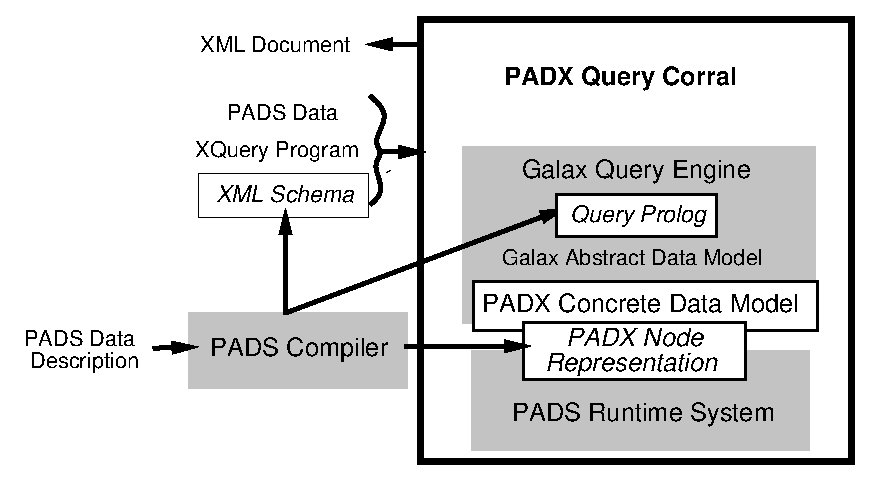
\epsfig{file=padx-arch.ps,width=0.47\textwidth}
\end{center}
\caption{\padx{} Architecture}
\label{figure:padx-arch}
\end{figure}

Figure~\ref{figure:padx-arch} depicts the \padx{} architecture.  From
a \pads{} description, the compiler generates an XML Schema
description that specifies the virtual XML view of the corresponding
\pads{} data; an XQuery prolog that imports the corresponding schema
and that associates the input data with the correct schema type; and a
type-specific library that maintains the information necessary to
support the \padx{} data model.

An instance of the \padx{} runtime system, called the ``query
corral'', consists of the \Galax{} query engine, a type-specific query
prolog, the \padx{} implementation of the \Galax{} data model, a
type-specific \padx{} library, and the \pads{} runtime system.  Note
that the resulting query corral is \emph{specialized} for a particular
\pads{} description.  From the query prolog, it imports the XML Schema
that corresponds to the underlying type-specific library, i.e., it
does permit the query writer to import an arbitrary schema.  This
restriction guarantees that the XQuery program is typed with respect
to the correct XML Schema and that the underlying data model is an
instance of the specified XML Schema.  At runtime, the query corral
takes an XQuery program and a \pads{} data source and produces the
query result in XML.  We discuss the problem of producing native
\pads{} values in Section~\ref{section:future}. 

Section~\ref{section:pads} describes the output of the \pads{}
compiler.  Here, we focus on the mapping from a description to XML
Schema and on the features of the type-specific data model.

\subsection{Virtual XML view of PADS data}

We use the fragment of the XML Schema in
Figure~\ref{figure:dibbler-schema}, which corresponds to the
description in Figure~\ref{figure:dibbler}, to illustrate the mapping
of a \pads{} description to XML Schema.
\begin{figure*}
\begin{small}
\begin{code}
<xs:schema targetNamespace="\kw{file:/example/sirius.p}"
           xmlns="file:/example/sirius.p"
           xmlns:xs="http://www.w3.org/2001/XMLSchema"
           xmlns:p="http://www.padsproj.org/pads.xsd">
<xs:import namespace = "http://www.padsproj.org/pads.xsd".../>
...
<xs:complexType name="\kw{order_header_t}">
 <xs:sequence>
  <xs:element name="\kw{order_num}"     type="\kw{p:val_Puint32}"/>
  <xs:element name="\kw{att_order_num}" type="\kw{p:val_Puint32}"/>
  <xs:element name="\kw{ord_version}"   type="\kw{p:val_Puint32}"/>
  <!-- More local element declarations -->
  <xs:element name="\kw{pd}"            type="\kw{p:PStruct_pd}" minOccurs="0"/>
 </xs:sequence>
</xs:complexType>
<!-- More complex type declarations -->
<xs:complexType name="\kw{orders_t}">
 <xs:sequence>
  <xs:element name="\kw{elt}"    type="\kw{order_t}" maxOccurs="unbounded"/>
  <xs:element name="\kw{length}" type="\kw{p:Puint32}"/>
  <xs:element name="\kw{pd}"     type="\kw{p:Parray_pd}" minOccurs="0"/>
 </xs:sequence>
</xs:complexType>
...
<xs:element name="PSource" type="summary"/>
</xs:schema>
\end{code}
\end{small}
\caption{Fragment of XML Schema for \dibbler{} \pads{} description.}
\label{figure:dibbler-schema}
\end{figure*}

``Error-aware'' mapping from PADS type system to isomorphic XML
Schema. 
\begin{small}
\begin{code}
<xs:simpleType name="Puint32">
  <xs:restriction base="xs:unsignedInt"/>
</xs:simpleType>
<xs:complexType name="\kw{val_Puint32}">
  <xs:\kw{choice}>
   <xs:element name="\kw{val}" type="\kw{p:Puint32}"/>
   <xs:element name="\kw{pd}"  type="\kw{p:Pbase_pd}"/>
  </xs:\kw{choice}>
</xs:complexType>
<xs:complexType name="\kw{Pbase_pd}">
 <xs:sequence>
   <xs:element name="\kw{pstate}"  type="\kw{p:Pflags_t}"/>
   <xs:element name="\kw{errCode}" type="\kw{p:PerrCode_t}"/>
   <xs:element name="\kw{loc}"     type="\kw{p:Ploc_t}"/>
 </xs:sequence>
</xs:complexType>
\end{code}
\end{small}

Each compound type is mapped to an XML Schema complex type.

Each base type is mapped to an XML Schema simple type.  Since the base
types do not change, the corresponding XML Schema types are defined
once in \cd{pads.xsd}, which is imported into all generated schemata. 

  One-to-one mapping
from PADS base types to XML Schema simple types.  Field in compound
types are realized as local elements in XML Schema. 

All the compound types are annotated with an optional parse-descriptor
(absent if no errors occured).  Allows users to query error
structures, which may be most important data.  Other types annotated
with corresponding fields from PADS rep, e.g., arrays have a length. 

Extra level of indirection in representation of arrays---wrap each
item in an element. 

Extra level of indirection for base types: must contain the value of
the base type and an optional parse-descriptor, if an error has
occurred. 

We don't take complete advantage of XML Schema, e.g., Penum types
could be modeled by XML Schema enumeration simple types, but currently
unsupported.

Example of query prolog. 
\begin{figure*}
\begin{small}
\begin{code}
import schema default element namespace "\kw{file:/example/sirius.p}";
declare variable \kw{$pads} as \kw{document-node(PSource)} external; 
\end{code}
\end{small}
\caption{\padx{} generated query prolog}
\label{figure:padx-query-prolog}
\end{figure*}

How to access data files:  fn:doc("pads:/example/sirius.data");

\subsection{Physical Data Model}

% Part of PADX implementation are generic functions that implement data
% model accessors.  PADS compiler generates type-specific functions for
% walking virtual XML tree.  Relate back to type-specific library
% functions mentioned in last section.

% Implementation of Galax's Abstract Tree Model.

% Minimum necessary to implement Galax DM:

% 1. Generic implementations of the DM accessors: axis::node-test(), children(),
%    attributes(), name(), etc. 

% 2. On PADX-side, we have a virtual handle for each node in the XML
%    tree--we call that a node rep.  Node rep contains pads handle
%    (maintains state for PADS parser); type-specific vtable of DM
%    accessors; other stuff...

%    Give example of vtable for event\_t and possibly code for
%    kthChildByName. 

In order to export \pads data as XML, we wrap data in {\em node}
datastructures containing all the information relevant to XML. Handles
to these nodes are then passed to \galax which can invoke very simple
queries on the node, such as ``what is your name? give me a list of
your children, etc.''  Within \galax, the interface with pads is
wrapped in a module that exports the \galax Data Model interface to
the \galax query engine.

The physical data model provides the means to query \pads data by
walking a virtual XML tree.  At the core of the physical data model
are the \cd{node} data structure and the generic node interface.
Together, these play the same role as an abstract class in C++ and
Java. They specify only common fields used by all nodes, and the
required accessor methods. They do not, however, provide any method
implementations. They are fixed elements of the system, independant of
any particular \pads{} types.

\begin{figure*}
{\small
\begin{verbatim}
nodeRep      PADX_generic_parent      (nodeRep n)

const char*  PADX_generic_name        (nodeRep n)
const char*  PADX_generic_kind        (nodeRep n)
item         PADX_generic_typed_value (nodeRep n)
const char*  PADX_generic_string_value(nodeRep n)

nodeRep      PADX_generic_kth_child         (nodeRep n, childIndex idx)
nodeRep      PADX_generic_kth_child_named   (nodeRep n, childIndex idx, 
                                             const char *name)
\end{verbatim}
}
\caption{The generic node interface}
\label{fig:generic-node-interface}
\end{figure*}

The generic node interface defines the functions that are available to the
\pads{} data model implementation for use on nodes. The relevant portions of
this interface are shown in \figref{fig:generic-node-interface}.

The {\tt kth-child} function returns the kth child of the node
starting from zero. The {\tt kth-child-named} function returns the node's kth
child with the specified name. This function is most relevant to
arrays, where all of the elements are given the same name ``elt.''
For both functions, {\tt NULL} is a valid result, indicating that the
requested child does not exist.

\begin{figure}
{\small
\begin{verbatim}
struct PDCI_node_s {
  const char              *name;
  const char              *kind;
  PDCI_node_t             *parent;

  void                    *m;
  void                    *pd;
  void                    *rep;

  const PDCI_vtable_t     *vt;
  P_t                     *pads;
  ...
}
\end{verbatim}
}
\caption{The node structure}
\label{fig:node-struct}
\end{figure}

The basic contents of the \cd{node} data structure are shown in
\figref{fig:node-struct}. All nodes have a name and a kind, stored as
C-strings. Additionally, all nodes but the document node have a parent
in the document, hence the parent field that points to another node.
Next we have the mask, representation and parse-descriptor fields. As
these elements of the node are type-specific, they are all typed as
\vptr.

Next we have the pointer to the node's virtual table, {\tt vt}. The
virtual functions will often need a valid \pads handle to execute
correctly. Therefore, we also include a pads handle field in each
node.

\subsubsection{Node implementations}
The PADS compiler generates the type-specific implementations of the
node functions, along with the other type-specific tools.  The
type-specific knowledge available at compile time is used not only to
manipulate the node's data appropriately but also to select the (type)
correct implementations of children nodes, when necessary.  For
example, for structures, the children are the parse-descriptor and the
fields of the structure, each with their own type and corresponding
node implementation.  For arrays, the children are the
parse-descriptor, the array length, and a list of nodes with name
``elt,'' corresponding to the elements of the array. The
parse-descriptor is accessed through an implementation for array pds,
the length field through an implementation for 32-bit integers, and
each of the elements with the implementation appropriate to the
particular element type of the array. Other datatypes are analagous.

It is important to note that the XML representations of \pads data
integrate each datastructure's parse-descriptor with the data,
exporting it as a child of the datastructure itself. This design
allows queries to select (or ignore) nodes based on the contents of
their parse-descriptors in an easy and efficient manner. It also means
that their are a fixed number of pd node implementations (approx. one for
each type constructor), as opposed to the unlimited number of data
node implementations, generated fresh for each new \pads{} type.

In order to support the full range of \pads datatypes,
the node data structure is designed using ``{\tt void *}
polymorphism.'' That is, anywhere that the node architecture is not
specific to a particular type, we use a {\tt void *} type. In this
way, we can write type-neutral code to manipulate data nodes. For
example, the rep and pd pointers in each node are typed as {\tt void
  *}. 

Each type-specific implementation will (down)cast such pointers to the
appropriate type before use, relying on the (assumed) invariant that
no only code specific to that type has manipulated those pointers.

\subsubsection{Data input strategies: when to actually read from PADS data?}

The flexibility of the node interface goes beyond support for
arbitrary \pads{} types. It also allows us, for each type, to support
alternative implementations of the interface. We take advantage of
this flexibility to support multiple data input strategies: bulk-read
and two forms of on-demand read.

\begin{enumerate}
\item Bulk read: Materialize entire PADS representation, populate all of the PADS
reps.  Then PADX DM lazily invoked the DM accessors over this data.
Problem: if data is big, it's all sitting in memory, even if the query
only touches a fragment of the virtual XML tree.

\item On-demand, sequential read: same as smart but does not preserve meta-data.
   Does not permit multiple scans of data source. 

\item On-demand, random access read: 
Many common queries permit sequential, streamed access to underlying
XML source.  Give an example.  

Smart node rep, preserves meta-data about previously read records, but
re-uses memory for reading next item.  This rep permits multiple scans
of input (semantic problem is that DM must preserve node identity),
but slowly. 

Heuristic: records are a good level of granularity to read.   Each
smart node corresponds to one record.  When next smart node is
accessed, a little meta-data is preserved: the node rep and the
records location in the file (so we can re-read it if necessary).
\end{enumerate}

Put in PADX signatures for constructing a new node and accessing
kthChild. 

Something about query evaluation:
Although we have not explored custom evaluation plans 
Galax's algebra or optimizer are particularly interesting in the 
\padx{}, we expect to do so 

%%% Local Variables: 
%%% mode: latex
%%% TeX-master: "paper"
%%% End: 

\section{Performance}
\label{section:performance}

\subsection{Materialization and Loading}

Hypothesis: bulk loading should not scale for increasing document size
(limits of main memory).  Show that smart/linear does scale.

The flexibility of the node interface goes beyond support for
arbitrary \pads{} types. It also allows us, for each type, to support
alternative implementations of the interface. We take advantage of
this flexibility to support multiple data input strategies: bulk-read
and two forms of on-demand read.

\begin{enumerate}
\item Bulk read: Materialize entire PADS representation, populate all of the PADS
reps.  Then PADX DM lazily invoked the DM accessors over this data.
Problem: if data is big, it's all sitting in memory, even if the query
only touches a fragment of the virtual XML tree.

\item On-demand, sequential read: same as smart but does not preserve meta-data.
   Does not permit multiple scans of data source. 

\item On-demand, random access read: 
Many common queries permit sequential, streamed access to underlying
XML source.  Give an example.  

Smart node rep, preserves meta-data about previously read records, but
re-uses memory for reading next item.  This rep permits multiple scans
of input (semantic problem is that DM must preserve node identity),
but slowly. 

Heuristic: records are a good level of granularity to read.   Each
smart node corresponds to one record.  When next smart node is
accessed, a little meta-data is preserved: the node rep and the
records location in the file (so we can re-read it if necessary).
\end{enumerate}

Put in PADX signatures for constructing a new node and accessing
kthChild. 

Something about query evaluation:
Although we have not explored custom evaluation plans 
Galax's algebra or optimizer are particularly interesting in the 
\padx{}, we expect to do so 

\subsection{Querying}

Give examples of queries that analyst cares about. 

Example of query that can be evaluated in single scan over data
source, but is currently not 

Database person would balk at this point!  Why aren't you just loading
this data into a real database, building indices and getting good
query performance?  B/c data is ephmeral, queries are ephmeral, but
analyst/programmer should profit from disciplined access/querying of
their data.  Don't abandon them to Perl. 



\paragraph*{Dealing with errors.}  
In 1967, Gold~\cite{gold:inference}
proved that learning a grammar for any remotely
sophisticated class of languages, such as the regular languages, 
is impossible if one is only given positive 
example data.\footnote{A positive example is a data source
known to be in the grammar to be learned.  
A negative example is one known {\em not} to be in the target grammar.
Learning with positive examples and negative examples is possible.
Unfortunately, given that data analysts are unlikely to have access to
ad hoc data that they know {\em does not} 
satisfy the format they are interested in learning,
we are forced to tackle the more difficult problem of learning from 
positive examples only.}
Given this negative theoretical result, and the practical fact
that it is hard to be sure that training data
is sufficiently rich to witness all possible variation in the data,
errors in inference are inevitable.  Fortunately, however, detecting
and recovering from errors in ad hoc data is one of the primary strengths
of the \pads{} system.  

To determine exactly how accurate an
inferred description is on any new data source, a user may run the
accumulator tool.  This tool catalogs exactly how many deviations
from the description there were overall in the data source
as well as the error rate in every individual field.
Hence, using this tool, a programmer can immediately and reliably
determine the effectiveness of inference for their data.
If there is a serious 
problem, the user can easily edit the generated description by hand
-- identification of a problem field, a minor
edit and recompilation of tools might just take 5 minutes.  Hence,
even imperfectly-generated descriptions have great value in terms of
improving programmer productivity.  Moreover, all \pads{}-generated 
parsers and tools
have error detection, representation and recovery techniques.
For instance, when converting data to \xml{}, errors encountered
are represented explicitly in the \xml{} document, allowing users to query
the data for errors if they choose.  Before graphing ad hoc data,
an analyst may use the accumulator tool to check if any errors occur
in the fields to be graphed.  If not, there is no reason to edit
the description at all -- graphing the correct fields may proceed 
immediately.

\paragraph*{Future work.}  
Discovering tokens like ``IP address'' and ``date'' is highly beneficial
as such tokens act as compact, highly 
descriptive, human-readable abstractions. 
Unfortunately, these tokens are also often 
mutually ambiguous.  For instance, an IP address, a 
floating point number 
and a phone number can all be represented as some number of digits 
separated by periods.  At the moment, we disambiguate between them 
in the same way that lex does, by taking the first, longest match. 
In select cases, when we cannot disambiguate in the tokenization phase, we
try to correct problems using domain-specific rewriting rules in the 
structure refinement phase.    
To improve tokenization in the future, we plan to look at learning
probabilistic models of a broad range of token types.  
We also
intend to explore finding new tokens from the data itself,
possibly by identifying abrupt changes in entropy~\cite{hutchens98finding}.

%From an experimental perspective,

% Hence, while our system allows users to
% customize the tokenization scheme through a configuration file,
% this customization requires work, and 
% for the computational biologist not accustomed to writing or 
% reading regular expressions, it creates a barrier to usage.  
% Moreover,
% since tokenization ambiguities are often unavoidable, even after tweaking
% tokenization configurations, system results
% are dependent upon our simplistic disambiguation 
% scheme.\footnote{We disambiguate
% like lex does, taking the first, longest match in the token list.}  
% Indeed, to avoid ambiguities that arise from having
% floating-point numbers be tokens, we do not identify floats during
% the tokenization face, but instead introduce floats through a number of 
% custom
% rewriting rules in the rewriting phase.  

% At the moment, we see two possible solutions to this problem.  The
% first solution is to attempt to identify new tokens from the data 
% source being learned, perhaps by identifying significant changes in entropy
% as suggested by.  This 

% thoughts on problems with tokenization; information theory; partial
% descriptions; user interface; recursion; more experimentation with a
% broader range of formats


\bibliographystyle{abbrv}
\small
\bibliography{../pads,../galax} 
\end{document}

